\documentclass[11pt]{article}
\usepackage[margin=0.78in]{geometry}
\usepackage{amsmath,amssymb,amsthm}
\usepackage[T1]{fontenc}
\usepackage{graphicx}
\usepackage[hidelinks]{hyperref}
\usepackage{microtype}
\usepackage{booktabs}

\newtheorem{theorem}{Theorem}
\newcommand{\xor}{\mathbin{\oplus}}

\title{A 32-Point Counterexample to the Additive--XOR Conjecture}
\author{fa\_banach\_001 / agent\_lane\_00}
\date{17 August 2026}

\begin{document}
\maketitle
\vspace{-1em}

\noindent\textbf{Status: candidate full counterexample, likely valid,}\\
\textbf{to the $B_n^\sigma$ conjecture in arXiv:math/0308091.}

\section{The conjecture}

Write $[N]=\{0,1,\ldots,N-1\}$ and let $\xor$ denote bitwise XOR.  For a
permutation $\sigma$ of $[2^n]$, Hinrichs and Wenzel define
\[
 B_n^\sigma=\{(k,l)\in[2^n]^2:k+l<2^n,
 \ \sigma(k)\xor\sigma(l)=\sigma(k+l)\}.
\]
They observe that $\#B_n^{\mathrm{id}}=3^n$, verify the upper bound for all
permutations when $n\leq4$, and conjecture that
$\#B_n^\sigma\leq3^n$ for every $n$ and every permutation
\cite[p.~17]{HW}.

\begin{center}
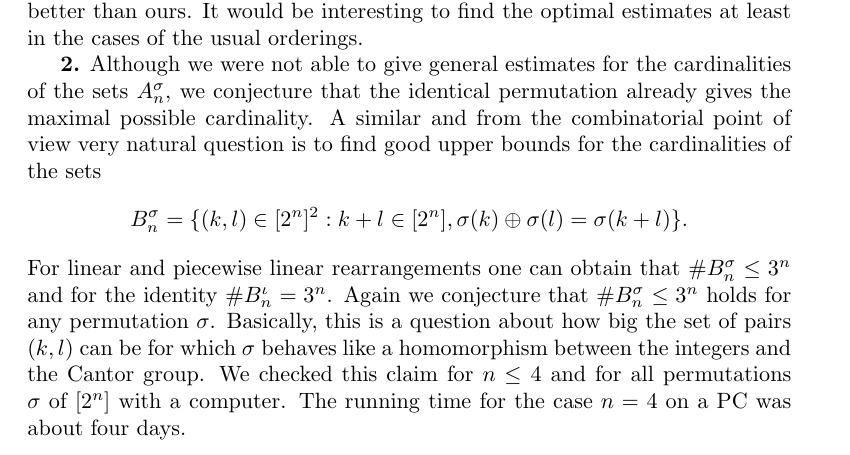
\includegraphics[width=0.93\textwidth]{figures/b_conjecture.png}
\end{center}

\section{Proof intuition}

The conjectured bound first fails at the next unchecked dimension.  An exact
local search at $n=5$ found a permutation with six more agreements than the
identity.  Postcomposition by an invertible linear map of the XOR group does
not change any agreement and turns the search output into the compact table
below.  The finite base count is certified by listing all 32 sum-fibre
counts.  The counterexample then lifts to every larger dimension: retain the
permutation on the lowest five bits and leave all higher bits fixed.  A carry
out of the low block makes the high-bit equality impossible by parity; with
no carry, each additional bit has the usual three choices.

\section{Counterexample and infinite lift}

Define $q:[32]\to[32]$ by the following table.
{\small
\[
\begin{array}{c|rrrrrrrrrrrrrrrr}
k&0&1&2&3&4&5&6&7&8&9&10&11&12&13&14&15\\ \hline
q(k)&0&1&2&3&4&11&10&9&8&15&14&13&12&19&18&5
\end{array}
\]}
{\small
\[
\begin{array}{c|rrrrrrrrrrrrrrrr}
k&16&17&18&19&20&21&22&23&24&25&26&27&28&29&30&31\\ \hline
q(k)&16&7&6&25&24&27&26&29&28&31&30&17&22&23&20&21
\end{array}
\]}

\begin{theorem}\label{thm:main}
The displayed $q$ is a permutation and
\[
 \#B_5^q=249>243=3^5.
\]
More generally, for every $n\geq5$, put $m=n-5$, write uniquely
$x=32b+a$ with $a\in[32]$ and $b\in[2^m]$, and define
\begin{equation}\label{eq:lift}
 \sigma_n(32b+a)=32b+q(a).
\end{equation}
Then $\sigma_n$ is a permutation of $[2^n]$ and
\[
 \#B_n^{\sigma_n}=249\,3^{n-5}>3^n.
\]
Thus the conjecture is false in every dimension $n\geq5$.
\end{theorem}

\begin{proof}
The displayed row of values contains each integer from 0 to 31 exactly once,
so $q$ is a permutation.  For $s\in[32]$ define the fibre count
\[
 c_s=\#\{a\in[0,s]:q(a)\xor q(s-a)=q(s)\}.
\]
Direct substitution in the displayed table gives, in blocks of eight,
\[
\begin{array}{c|rrrrrrrr}
s&0&1&2&3&4&5&6&7\\ \hline
c_s&1&2&2&4&2&2&4&4\\[2pt]
s&8&9&10&11&12&13&14&15\\ \hline
c_s&8&4&6&6&10&2&4&6\\[2pt]
s&16&17&18&19&20&21&22&23\\ \hline
c_s&6&12&10&6&6&10&12&8\\[2pt]
s&24&25&26&27&28&29&30&31\\ \hline
c_s&8&12&14&10&8&14&14&32
\end{array}
\]
Their sum is
\[
 \#B_5^q=\sum_{s=0}^{31}c_s=249.
\]
For comparison, under the identity permutation a decomposition $s=a+c$ is
good exactly when the binary supports of $a$ and $c$ are disjoint.  Each 1-bit
of $s$ can be assigned to either summand, so the corresponding fibre has
$2^{\operatorname{popcount}(s)}$ elements.  Therefore
\[
 \#B_n^{\mathrm{id}}
 =\sum_{s<2^n}2^{\operatorname{popcount}(s)}=(1+2)^n=3^n.
\]
This proves the strict inequality in the base case.

It remains to prove the lifting formula.  Let
\[
 x=32b+a,\qquad y=32d+c
\]
with $a,c\in[32]$ and $b,d\in[2^m]$, and assume $x+y<2^n$.  If
$a+c\geq32$, then comparison of the high blocks in
$\sigma_n(x)\xor\sigma_n(y)=\sigma_n(x+y)$ would require
\[
 b\xor d=b+d+1.
\]
The two sides have opposite parity, so no such pair is good.

If $a+c<32$, the equality separates into
\[
 q(a)\xor q(c)=q(a+c),
 \qquad
 b\xor d=b+d.
\]
The first condition has 249 ordered solutions $(a,c)$.  The second says that
$b$ and $d$ have disjoint binary supports.  Independently at each of the $m$
high bits, the pair of bits is $(0,0)$, $(1,0)$, or $(0,1)$, giving exactly
$3^m$ solutions.  Such a carry-free high sum is automatically below $2^m$.
Hence
\[
 \#B_n^{\sigma_n}=249\,3^m=249\,3^{n-5}
 >243\,3^{n-5}=3^n,
\]
as claimed.
\end{proof}

\section*{Verification, novelty, and scope}

The accompanying verifier checks that the table is a permutation, reconstructs
all 32 fibre counts and their sum using integer XOR, verifies the identity
benchmark, and exhaustively checks the lifted counts through $n=10$.  These
finite checks are not used for the all-$n$ lifting argument, which is proved
above by carry and parity analysis.

The paper states a separate conjecture that the identity maximizes the
four-term cardinality $\#A_n^\sigma$.  The present $q$ has
$\#A_5^q=6912<7776=\#A_5^{\mathrm{id}}$, so this packet makes no claim about
that conjecture.

A bounded novelty search checked the run indexes, the exact conjecture,
author/title searches, and the source's citation graph.  OpenAlex lists one
later citation, Sanders' arXiv:1901.03109, which proves full Walsh--trigonometric
nonequivalence by a different additive-combinatorial route but does not state
this finite conjecture or the counterexample.  No later explicit resolution
was located.  Novelty is therefore provisional pending expert search.

\begin{thebibliography}{9}
\bibitem{HW}
A. Hinrichs and J. Wenzel,
\emph{On the non-equivalence of rearranged Walsh and trigonometric systems in
$L_p$}, Studia Mathematica 159 (2003), 435--451;
arXiv:math/0308091.
\end{thebibliography}

\end{document}
